% Created by tikzDevice version 0.12.3 on 2019-12-11 20:53:33
% !TEX encoding = UTF-8 Unicode
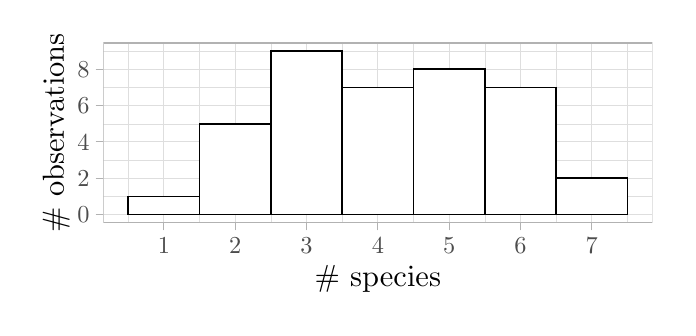
\begin{tikzpicture}[x=1pt,y=1pt]
\definecolor{fillColor}{RGB}{255,255,255}
\path[use as bounding box,fill=fillColor,fill opacity=0.00] (0,0) rectangle (231.26,101.18);
\begin{scope}
\path[clip] (  0.00,  0.00) rectangle (231.26,101.18);
\definecolor{drawColor}{RGB}{255,255,255}
\definecolor{fillColor}{RGB}{255,255,255}

\path[draw=drawColor,line width= 0.6pt,line join=round,line cap=round,fill=fillColor] (  0.00,  0.00) rectangle (231.26,101.18);
\end{scope}
\begin{scope}
\path[clip] ( 27.31, 30.69) rectangle (225.76, 95.68);
\definecolor{fillColor}{RGB}{255,255,255}

\path[fill=fillColor] ( 27.31, 30.69) rectangle (225.76, 95.68);
\definecolor{drawColor}{gray}{0.87}

\path[draw=drawColor,line width= 0.1pt,line join=round] ( 27.31, 40.20) --
	(225.76, 40.20);

\path[draw=drawColor,line width= 0.1pt,line join=round] ( 27.31, 53.33) --
	(225.76, 53.33);

\path[draw=drawColor,line width= 0.1pt,line join=round] ( 27.31, 66.46) --
	(225.76, 66.46);

\path[draw=drawColor,line width= 0.1pt,line join=round] ( 27.31, 79.59) --
	(225.76, 79.59);

\path[draw=drawColor,line width= 0.1pt,line join=round] ( 27.31, 92.72) --
	(225.76, 92.72);

\path[draw=drawColor,line width= 0.1pt,line join=round] ( 36.33, 30.69) --
	( 36.33, 95.68);

\path[draw=drawColor,line width= 0.1pt,line join=round] ( 62.11, 30.69) --
	( 62.11, 95.68);

\path[draw=drawColor,line width= 0.1pt,line join=round] ( 87.88, 30.69) --
	( 87.88, 95.68);

\path[draw=drawColor,line width= 0.1pt,line join=round] (113.65, 30.69) --
	(113.65, 95.68);

\path[draw=drawColor,line width= 0.1pt,line join=round] (139.43, 30.69) --
	(139.43, 95.68);

\path[draw=drawColor,line width= 0.1pt,line join=round] (165.20, 30.69) --
	(165.20, 95.68);

\path[draw=drawColor,line width= 0.1pt,line join=round] (190.97, 30.69) --
	(190.97, 95.68);

\path[draw=drawColor,line width= 0.1pt,line join=round] (216.74, 30.69) --
	(216.74, 95.68);

\path[draw=drawColor,line width= 0.3pt,line join=round] ( 27.31, 33.64) --
	(225.76, 33.64);

\path[draw=drawColor,line width= 0.3pt,line join=round] ( 27.31, 46.77) --
	(225.76, 46.77);

\path[draw=drawColor,line width= 0.3pt,line join=round] ( 27.31, 59.90) --
	(225.76, 59.90);

\path[draw=drawColor,line width= 0.3pt,line join=round] ( 27.31, 73.03) --
	(225.76, 73.03);

\path[draw=drawColor,line width= 0.3pt,line join=round] ( 27.31, 86.16) --
	(225.76, 86.16);

\path[draw=drawColor,line width= 0.3pt,line join=round] ( 49.22, 30.69) --
	( 49.22, 95.68);

\path[draw=drawColor,line width= 0.3pt,line join=round] ( 74.99, 30.69) --
	( 74.99, 95.68);

\path[draw=drawColor,line width= 0.3pt,line join=round] (100.77, 30.69) --
	(100.77, 95.68);

\path[draw=drawColor,line width= 0.3pt,line join=round] (126.54, 30.69) --
	(126.54, 95.68);

\path[draw=drawColor,line width= 0.3pt,line join=round] (152.31, 30.69) --
	(152.31, 95.68);

\path[draw=drawColor,line width= 0.3pt,line join=round] (178.08, 30.69) --
	(178.08, 95.68);

\path[draw=drawColor,line width= 0.3pt,line join=round] (203.86, 30.69) --
	(203.86, 95.68);
\definecolor{drawColor}{RGB}{0,0,0}

\path[draw=drawColor,line width= 0.6pt,line cap=rect,fill=fillColor] ( 36.33, 33.64) rectangle ( 62.11, 40.20);

\path[draw=drawColor,line width= 0.6pt,line cap=rect,fill=fillColor] ( 62.11, 33.64) rectangle ( 87.88, 66.46);

\path[draw=drawColor,line width= 0.6pt,line cap=rect,fill=fillColor] ( 87.88, 33.64) rectangle (113.65, 92.72);

\path[draw=drawColor,line width= 0.6pt,line cap=rect,fill=fillColor] (113.65, 33.64) rectangle (139.43, 79.59);

\path[draw=drawColor,line width= 0.6pt,line cap=rect,fill=fillColor] (139.43, 33.64) rectangle (165.20, 86.16);

\path[draw=drawColor,line width= 0.6pt,line cap=rect,fill=fillColor] (165.20, 33.64) rectangle (190.97, 79.59);

\path[draw=drawColor,line width= 0.6pt,line cap=rect,fill=fillColor] (190.97, 33.64) rectangle (216.74, 46.77);
\definecolor{drawColor}{gray}{0.70}

\path[draw=drawColor,line width= 0.6pt,line join=round,line cap=round] ( 27.31, 30.69) rectangle (225.76, 95.68);
\end{scope}
\begin{scope}
\path[clip] (  0.00,  0.00) rectangle (231.26,101.18);
\definecolor{drawColor}{gray}{0.30}

\node[text=drawColor,anchor=base east,inner sep=0pt, outer sep=0pt, scale=  0.88] at ( 22.36, 30.61) {0};

\node[text=drawColor,anchor=base east,inner sep=0pt, outer sep=0pt, scale=  0.88] at ( 22.36, 43.74) {2};

\node[text=drawColor,anchor=base east,inner sep=0pt, outer sep=0pt, scale=  0.88] at ( 22.36, 56.87) {4};

\node[text=drawColor,anchor=base east,inner sep=0pt, outer sep=0pt, scale=  0.88] at ( 22.36, 70.00) {6};

\node[text=drawColor,anchor=base east,inner sep=0pt, outer sep=0pt, scale=  0.88] at ( 22.36, 83.13) {8};
\end{scope}
\begin{scope}
\path[clip] (  0.00,  0.00) rectangle (231.26,101.18);
\definecolor{drawColor}{gray}{0.70}

\path[draw=drawColor,line width= 0.3pt,line join=round] ( 24.56, 33.64) --
	( 27.31, 33.64);

\path[draw=drawColor,line width= 0.3pt,line join=round] ( 24.56, 46.77) --
	( 27.31, 46.77);

\path[draw=drawColor,line width= 0.3pt,line join=round] ( 24.56, 59.90) --
	( 27.31, 59.90);

\path[draw=drawColor,line width= 0.3pt,line join=round] ( 24.56, 73.03) --
	( 27.31, 73.03);

\path[draw=drawColor,line width= 0.3pt,line join=round] ( 24.56, 86.16) --
	( 27.31, 86.16);
\end{scope}
\begin{scope}
\path[clip] (  0.00,  0.00) rectangle (231.26,101.18);
\definecolor{drawColor}{gray}{0.70}

\path[draw=drawColor,line width= 0.3pt,line join=round] ( 49.22, 27.94) --
	( 49.22, 30.69);

\path[draw=drawColor,line width= 0.3pt,line join=round] ( 74.99, 27.94) --
	( 74.99, 30.69);

\path[draw=drawColor,line width= 0.3pt,line join=round] (100.77, 27.94) --
	(100.77, 30.69);

\path[draw=drawColor,line width= 0.3pt,line join=round] (126.54, 27.94) --
	(126.54, 30.69);

\path[draw=drawColor,line width= 0.3pt,line join=round] (152.31, 27.94) --
	(152.31, 30.69);

\path[draw=drawColor,line width= 0.3pt,line join=round] (178.08, 27.94) --
	(178.08, 30.69);

\path[draw=drawColor,line width= 0.3pt,line join=round] (203.86, 27.94) --
	(203.86, 30.69);
\end{scope}
\begin{scope}
\path[clip] (  0.00,  0.00) rectangle (231.26,101.18);
\definecolor{drawColor}{gray}{0.30}

\node[text=drawColor,anchor=base,inner sep=0pt, outer sep=0pt, scale=  0.88] at ( 49.22, 19.68) {1};

\node[text=drawColor,anchor=base,inner sep=0pt, outer sep=0pt, scale=  0.88] at ( 74.99, 19.68) {2};

\node[text=drawColor,anchor=base,inner sep=0pt, outer sep=0pt, scale=  0.88] at (100.77, 19.68) {3};

\node[text=drawColor,anchor=base,inner sep=0pt, outer sep=0pt, scale=  0.88] at (126.54, 19.68) {4};

\node[text=drawColor,anchor=base,inner sep=0pt, outer sep=0pt, scale=  0.88] at (152.31, 19.68) {5};

\node[text=drawColor,anchor=base,inner sep=0pt, outer sep=0pt, scale=  0.88] at (178.08, 19.68) {6};

\node[text=drawColor,anchor=base,inner sep=0pt, outer sep=0pt, scale=  0.88] at (203.86, 19.68) {7};
\end{scope}
\begin{scope}
\path[clip] (  0.00,  0.00) rectangle (231.26,101.18);
\definecolor{drawColor}{RGB}{0,0,0}

\node[text=drawColor,anchor=base,inner sep=0pt, outer sep=0pt, scale=  1.10] at (126.54,  7.64) {\# species};
\end{scope}
\begin{scope}
\path[clip] (  0.00,  0.00) rectangle (231.26,101.18);
\definecolor{drawColor}{RGB}{0,0,0}

\node[text=drawColor,rotate= 90.00,anchor=base,inner sep=0pt, outer sep=0pt, scale=  1.10] at ( 13.08, 63.18) {\# observations};
\end{scope}
\end{tikzpicture}
